% presentable.tex -- storygit, the outward-facing document.
% Compile: tectonic presentable.tex
\documentclass[11pt,a4paper]{article}

\usepackage[T1]{fontenc}
\usepackage[utf8]{inputenc}
\usepackage{charter}
\usepackage[charter]{mathdesign}
\usepackage[margin=2.6cm]{geometry}
\usepackage{microtype}
\usepackage{graphicx}
\usepackage{booktabs}
\usepackage{enumitem}
\usepackage{xcolor}
\usepackage{titlesec}
\usepackage{caption}
\usepackage[hidelinks]{hyperref}

\definecolor{sgink}{HTML}{2B2A28}
\definecolor{sgslate}{HTML}{5C5A55}
\definecolor{sgaccent}{HTML}{8C5A3C}
\definecolor{sgrule}{HTML}{D6D2C8}

\color{sgink}
\captionsetup{font=small, labelfont={small,it}, textfont=small}
\titleformat{\section}{\large\bfseries}{\thesection}{0.7em}{}
\titleformat{\subsection}{\normalsize\bfseries}{\thesubsection}{0.6em}{}
\setlist{itemsep=1pt, topsep=3pt, parsep=0pt}
\setlength{\parskip}{0.4em}
\setlength{\parindent}{0pt}

\newcommand{\storygit}{\textsf{storygit}}
\newcommand{\decision}[1]{\subsection{#1}}
\newcommand{\rejected}[1]{\textit{Rejected:} #1}

\title{\storygit\\[0.3em]\large Version control for story state}
\author{Arush Gumber}
\date{}

\begin{document}
\maketitle
\thispagestyle{empty}

\begin{abstract}
\noindent
\storygit{} is an AI-assisted storytelling system that develops a one-line premise into
a structured serial --- Story, Episodes, Scenes, Beats, Prose --- while keeping the
writer in authority over every change. Its claim is that the hard part of long-form
AI-assisted fiction is not generation but \emph{state}: what is true, who knows it,
what depends on it, and what a given edit therefore invalidates. \storygit{} models the
story as a versioned typed state graph, makes every AI action a reviewable diff against
it, propagates edits by \emph{marking} affected nodes rather than rewriting them,
checks continuity graph-first before it ever asks a model, and learns the writer's taste
from their accept, reject, and edit signals. This document states the problem, the
design, the decisions and their rejected alternatives, and the measurements.
\end{abstract}

\vspace{1em}

\section{The problem}

A writer starts with a sentence: \emph{a powerless orphan discovers an ability that
could change the balance of power in a world at war.} They want to end with a serial ---
tens or hundreds of episodes, coherent, in their voice, with the mechanics that make a
listener press \emph{next episode}. The naive form of AI assistance, prompt to story,
fails at this in five reliable ways.

\textbf{State drift.} Facts established early are forgotten or contradicted later. The
model has no ledger of what it has committed to, so episode~14 puts a character in a
city they left in episode~9. The sharpest version of this failure is
\emph{epistemic}: a character acts on information the story has never given them. A
reader forgives an inconsistent hair colour; they do not forgive a character who
somehow already knows the secret.

\textbf{Broken edit semantics.} The writer changes one scene. Either nothing downstream
responds --- the story now contains a contradiction nobody flagged --- or the system
regenerates the plan and destroys work the writer had already approved. Both come from
the same absence: nothing records what depends on what. Fabula's own study~\cite{mirowski2026fabula} reports
exactly this, from several writers independently.

\textbf{Agency erosion.} When the system proposes whole drafts, the writer's role
collapses into judging them. Fabula's participants described becoming ``an arbiter of
good or bad'' rather than an author~\cite{mirowski2026fabula}. That is a worse job than writing, and it is the
reason a tool can be impressive in a demo and unused in a month.

\textbf{Exploration overwhelm.} Offering more alternatives is not the same as offering
more choice. Unlabeled variants cost more to read than they save, and a writer will
stop opening them.

\textbf{No learning.} The thirtieth iteration repeats the first iteration's mistakes.
Nothing in the system is a model of \emph{this} writer's taste, so every correction has
to be made again.

To these, serialized audio fiction adds a sixth: \textbf{no serial mechanics}. Hooks,
cliffhangers, recaps, and the open threads a listener is waiting to see paid off are the
retention surface of the product, and a general-purpose story generator does not track
any of them.

\section{Thesis}

Treat the story as a \textbf{versioned, typed state graph}. Make every AI action a
\textbf{reviewable diff} against that graph rather than a block of replacement text.
Make dependencies \textbf{explicit}, so that an edit propagates by \emph{marking} what it
affected and never by rewriting it. Let the writer \textbf{own the objective}, in their
own words, rather than ranking against the system's. And \textbf{learn the writer's
taste} from the signals they are already producing --- what they accept, what they
reject, and how they edit.

The division of labour follows: \textbf{the AI handles coherence and mechanics; the human
handles taste, voice, and retention.}

Stated as a difference: Fabula is a chain of prompts with a user interface. \storygit{}
is a state machine with a learning loop. The chain is fast to build and pleasant to
demonstrate; the state machine is what survives episode~40.

\section{Fabula, and the gaps this exploits}
\label{sec:fabula}

Fabula~\cite{mirowski2026fabula} is the closest published system, and the immediate
predecessor of this design's questions; Dramatron~\cite{mirowski2023dramatron} and
Wordcraft~\cite{yuan2022wordcraft} are the hierarchical-generation and
writer-in-the-loop lines it builds on, and the creativity-support
literature~\cite{cherry2014csi} supplies the evaluation vocabulary.

\textit{[Written in chunk 2 --- summary of the Fabula system, its user study findings,
and the five gaps \storygit{} targets: no dependency tracking, no per-character
knowledge state, no learning from writer signals, no serial mechanics, and diversity
implemented as ``do not repeat the last suggestion''.]}

\section{Architecture}
\label{sec:architecture}

\textit{[Full system diagram and component walk-through --- chunk 6. Model routing
subsection --- chunk 2.]}

\section{The state model}
\label{sec:state}

Five things are stored, and everything else is derived from them.

\textbf{The plan tree.} Story, Episode, Scene, Beat, Prose. Every node carries the four
planning questions Fabula found writers actually use --- what happens, what the audience
learns, how they feel, where and when --- plus a review status
(\textsf{draft}, \textsf{accepted}, \textsf{locked}, \textsf{stale}) and, when stale, the
reason. Episode nodes add the serial mechanics: hook, cliffhanger, recap of the previous
episode, threads carried in and left out, writer-set goals, and a target length. Beat
nodes add \textsf{produces} and \textsf{consumes} --- the declared fact dependencies that
make propagation exact.

\textbf{The world graph.} Entities (characters, places, objects, factions) with an alias
table, and facts as edges between them. A fact carries a validity interval over the
global beat order, so a fact that changes does not overwrite its own history: Kael is in
Ashfall for beats 3 through 7 and elsewhere afterwards, and both are retrievable at their
own times. Predicates come from a closed vocabulary
(\textsf{location}, \textsf{alive}, \textsf{injury}, \textsf{possesses},
\textsf{relationship}, \textsf{relationship\_status}, \textsf{goal}, \textsf{secret},
\textsf{trait}, \textsf{faction}) plus a free-text \textsf{note}. Closed is what makes the
first layer of continuity checking a dictionary lookup rather than a model call.

\textbf{Epistemic edges.} \textsf{knows}(character, fact, since beat), tracked separately
from the facts themselves, because the difference between what is true and what a
character has been told is the single richest source of continuity errors in generated
fiction.

\textbf{The open-thread ledger.} Each thread records when it was opened and last
advanced, so ``you opened the sister subplot in episode 2 and have not touched it in
nine episodes'' is a query, not a judgement.

\textbf{The writer ledger.} Locks, hard constraints, style notes, writer-defined scoring
criteria in the writer's own words, rejected directions, and the coherent-to-surprising
dial. This is the object that keeps the human in authority, and everything in it is
visible and deletable --- including the rules the system mined from the writer's own
edits, which must never influence generation invisibly.

Provenance is recorded per sentence (\textsf{human}, \textsf{ai},
\textsf{ai\_edited\_by\_human}), because the interesting case is mixed: the AI proposed a
paragraph and the writer rewrote two sentences of it. A node-level flag would lose exactly
the information the writer cares about, and the authorship ratio shown in the interface
would be a lie.

\begin{figure}[t]
\centering
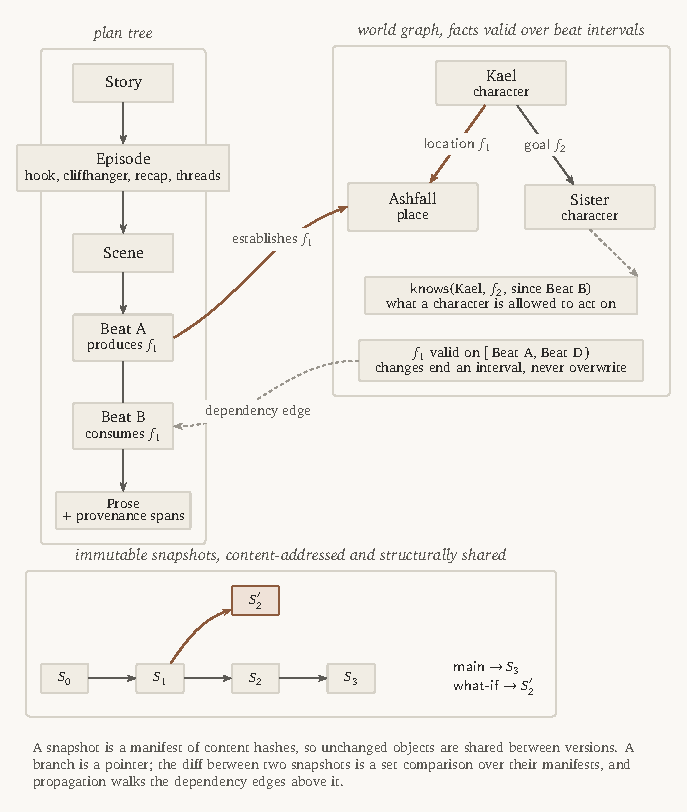
\includegraphics[width=0.95\textwidth]{diagrams/state_model.pdf}
\caption{The three stores and how they reference each other. The plan tree holds
structure; the world graph holds truth with validity intervals; snapshots hold history.
A beat's \textsf{produces} and \textsf{consumes} lists are the only dependency edges
propagation walks, which is what makes the walk exact.}
\label{fig:state-model}
\end{figure}

\subsection{Snapshots, branches, and why the project is called \storygit}

Every object is stored once under the SHA-256 of its canonical JSON. A snapshot is a
\emph{manifest}: a mapping from logical id to content hash, plus a parent pointer, the
author, and the intent line. A branch is a name pointing at a snapshot.

Three properties fall out for free. Versions are cheap: committing a change that touches
three nodes writes three object rows and one manifest, so a five-hundred-snapshot history
of a two-hundred-node story costs the changed nodes, not five hundred copies. Structural
diff needs no heuristics: what changed between two versions is a set comparison over two
manifests. And the whole thing is reproducible: identical content yields an identical
manifest, so ``apply the same diff twice and get the same hashes'' is a test rather than a
hope.

Merging is three-way at object granularity. Where only one side changed an object, that
side wins. Where both changed it differently, the merge returns a conflict. It never
guesses which version of a scene the author meant.

\section{The proposal engine}
\label{sec:proposals}

\textit{[Chunk 2: proposals as diffs, progressive levels, structured output. Chunk 3:
axis-conditioned sampling, MMR and DPP selection, the dial.]}

\section{Propagation}
\label{sec:propagation}

Dependency edges are declared, not inferred: a beat states the facts it establishes and
the facts it relies on, and an edge from beat $A$ to beat $B$ exists exactly when $B$
consumes something $A$ produced. When an accepted change alters or removes a fact, the
system walks the consumers transitively and \emph{marks} them. It never rewrites them.

Three rules make this safe to leave running.

\begin{enumerate}[label=\arabic*.]
\item \textbf{Locked nodes are never marked}, and the walk does not pass through them. A
locked beat is not going to change, so nothing it produces can change either. The
operational meaning of a lock is broader than that: every fact a locked node establishes
is exported into every subsequent prompt as a hard constraint.
\item \textbf{Human prose is flagged for review, not staled.} The system does not tell an
author that their own sentences are out of date; it tells them something they relied on
moved, and leaves the judgement where it belongs.
\item \textbf{Nothing is ever rewritten.} The writer chooses: regenerate (previewed as a
diff, respecting locks and current facts), edit by hand, or dismiss --- ``it still
works''. Regenerating a whole stale subtree exists, as an explicit, confirmed, previewed
action.
\end{enumerate}

Because the marks are emitted as ordinary status operations, staleness flows through the
same snapshot machinery as every other change. There is no side channel, and the history
shows why each node was marked and by which upstream fact.

The same walk, run against a candidate that has not been accepted, is what produces the
line the writer reads under every proposal: \emph{``would mark 2 downstream beats
stale''}. The blast radius is visible before the decision, not after it.

\section{Continuity checking}
\label{sec:continuity}

\textit{[Chunk 3: three layers --- deterministic graph checks, local NLI for free-text
facts, and an LLM soft judge --- with the recall each layer contributes and why the
order is deterministic-first.]}

\section{The preference layer}
\label{sec:preference}

\textit{[Chunk 4: exemplar retrieval, edit-pair mining, the contrastive voice model,
edit direction vectors, the Bradley-Terry preference head, and Thompson sampling over
safe and exploratory slots. Includes the honest paragraph about the data regime.]}

\section{Evaluation}
\label{sec:evaluation}

\textit{[Chunk 5: simulated writers with hidden weight vectors, injected ground-truth
contradictions, the metric definitions, the ablation table, and the curves.]}

\section{Decisions, and what was rejected}
\label{sec:decisions}

\decision{Diffs rather than replacement text}
Every AI action is a typed operation list against the current state, not a block of prose
that overwrites what was there. \rejected{Text-level replacement with a visual diff.} It
looks similar in the interface and is far weaker underneath: a text diff cannot say
``this introduces a character'', cannot be checked against the world graph before it is
applied, and cannot tell the writer what it would invalidate.

\decision{Declared dependencies rather than inferred ones}
A beat states what it produces and consumes; propagation walks those edges only.
\rejected{Inferring dependencies with a model.} A dependency oracle that is wrong ten
percent of the time makes every propagation result untrustworthy, which is worse than no
propagation at all --- the writer stops reading the marks. Embedding-similarity edges are
implemented, but as a clearly weaker ``maybe affected'' signal and as an ablation to
measure, never as the primary mechanism.

\decision{A closed predicate vocabulary}
Ten predicates plus a free-text escape hatch. \rejected{Open-vocabulary relation
extraction.} Closed predicates make the first checker layer a dictionary lookup and an
equality test --- free, instant, and never wrong for the wrong reason. The escape hatch
is exactly the set of facts that needs the more expensive NLI check, which is a useful
way to have partitioned the problem.

\decision{Content-addressed snapshots}
\rejected{Storing a full copy of the story per version, or an event log without
materialized states.} Full copies do not survive a few hundred snapshots. A pure event
log makes ``what is true right now'' a replay, and makes branch comparison hard.
Content addressing gives cheap versions, free structural sharing, and diff as set
arithmetic.

\decision{Marking rather than auto-repair}
\rejected{Automatically regenerating stale downstream nodes.} This is the single most
tempting feature in the system and the one that would destroy it. It is precisely what
Fabula's writers complained about, and the reason is not technical: a system that
rewrites approved work without asking cannot be trusted with a manuscript.

\decision{SQLite}
\rejected{Postgres.} One writer, one story, a few megabytes, and a file the author can
copy is the actual workload. Postgres buys concurrency this system does not have. What
would change at a serialized-fiction platform scale is discussed in the systems documentation.

\textit{[Further decisions --- provider routing, MMR versus DPP, the preference head's
feature set, the simulated-writer evaluation --- are added as their chunks land.]}

\section{Limitations}
\label{sec:limitations}

\textit{[Chunk 5: what the simulated-writer evaluation can and cannot measure; the data
regime for the preference layer; single-writer assumption; cost model.]}

\bibliographystyle{plain}
\bibliography{refs}

\end{document}
